\documentclass{beamer}
\usepackage[spanish]{babel}
\usepackage{graphicx}
\usepackage{xcolor}
\usepackage{latexsym}
\usepackage{amsmath}
\usepackage{amssymb}
\usepackage{multicol}
\usepackage{tikz}

\usetheme{Boadilla}

\newtheorem{Teorema}{Teorema}

\definecolor{myblue}{RGB}{80, 69, 190} 

\setlength{\parskip}{0.1cm}

\newcommand{\indc}[4]{
    \begin{frame}
        \frametitle{Índice}
        	\begin{enumerate}
            \setbeamercovered{transparent}
            \item<#1> Clave-Valor  
            \item<#2> Columnar      
            \item<#3> Documental    
            \item<#4> Grafo
        \end{enumerate}
    \end{frame}
}

\newcommand{\mytitle}[4]{
    \centering
    \vspace{0.1cm}
    
    {\Large \color{myblue} #1}

    \vspace{0.1cm}

    {\Large \color{myblue} #2}
    
    \vspace{0.5cm}
    
    {#3}
    
    \vspace{0.5cm}
    
    {\color{gray} #4}
    
    \vspace{0.5cm}
    
    {\today}
}

\title{Bases de datos NoSQL}
\author{Arroyo Joaquin \\ Belmonte Marina}

\begin{document}

\begin{frame}
    \mytitle
    {Bases de datos NoSQL}
    {Clase 1}
    {Arroyo Joaquin \\ Belmonte Marina}
    {Universidad Nacional de Rosario \\ Licenciatura en Ciencias de la Computación \\ Bases de Datos Avanzadas}
\end{frame}

\section{Introduccion}

\begin{frame}
    \frametitle{Resúmen}

    \begin{itemize}
        \item Repaso de Modelos NoSQL

         
        
        \item Implementaciones de Modelos NoSQL

        \begin{itemize}
            \item Redis
            \item Apache HBase
            \item MongoDB
            \item Neo4j
        \end{itemize}

         
        
        \item Dos artículos que estudian el rendimiento de bases de datos SQL versus NoSQL en aplicaciones reales
    \end{itemize}
    
\end{frame}

\section{Caracterización}

\begin{frame}
    \frametitle{Caracterización}

    ¿ Qué es una base de datos \textit{NoSQL} ?

     
    
    La definición más simple es: ``\textit{Una base de datos que no sigue el modelo relacional}''.

      

    Una gran cantidad de modelos se adaptan a dicha definición, es por esto que además presentan las siguientes características:

     
    
    \begin{itemize}
        \item Pueden correr fácilmente en clusters sin \textit{Single Point of Failure}.             
        \item Operan sin un esquema fijo, permitiendo agregar campos a los registros \textit{on-the-fly}.     
        \item Siguen el principio \textbf{BASE} (\textbf{B}asically \textbf{A}vailable, \textbf{S}oft State, \textbf{E}ventually Consistent)  
        \item Hacen incapié en el desempeño y la flexibilidad sobre la potencia de modelización y las consultas complejas.  
        \item Usualmente son nuevas y de software libre.
    \end{itemize}
    
\end{frame}

\section{¿Por qué NoSQL?}

\begin{frame}
    \frametitle{¿Por qué NoSQL?}

    Pero, ¿por qué surgen las bases de datos no relacionales?

     
    
    Principalmente por el crecimiento exponencial de la información, debido al uso de nuevas tecnologías en la sociedad.
    
     
    
    Dicho crecimiento es impulsado por

     
    
    \begin{itemize}
        \item Internet             
        \item Teléfonos móviles     
        \item Redes Sociales         
        \item etc.                   
    \end{itemize}

    Como consecuencia surgieron conceptos como

     

    \begin{itemize}
        \item Web 2.0
        \item Big Data
        \item Cloud Computing
    \end{itemize}
\end{frame}

\begin{frame}
    \frametitle{¿Por qué NoSQL?}

    Estos avances llevaron tanto a la industria como a la academia a replantearse el uso de los modelos relacionales debido a sus limitaciones naturales en el manejo de grandes cantidades de información.

     
    
    Se necesitaban (\textit{necesitan}) sistemas que escalen horizontalmente de manera sencilla.
    
     

    Se empiezan a investigar y desarrollar posibles alternativas por fuera de los modelos relacionales, que resuelvan estos problemas.
    
     

    Prinpalmente es por esto que surgen las \textit{Bases de Datos NoSQL}.
\end{frame}

\begin{frame}
    \frametitle{¿Por qué NoSQL? - Tecnologías vs NoSQL}

    \centering
    
    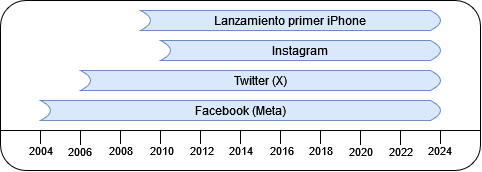
\includegraphics[width=0.65\textwidth]{diagramas/linea-temporal-tecno.png}

    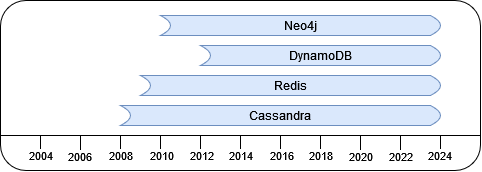
\includegraphics[width=0.65\textwidth]{diagramas/lineatemporal-nosql.png}
\end{frame}

\section{SQL vs NoSQL}

\section{SQL versus NOSQL}

\begin{frame}
    \frametitle{SQL vs NoSQL}

    Las principales diferencias entre estos dos modelos de datos son

     

    \begin{enumerate}
        \item \textbf{Estructura de los datos.}

        SQL usa el modelo relacional, esquemas rígidos.

        NoSQL no usa esquemas rígidos, da más flexibilidad.

         
        
        \item \textbf{Escalabilidad}

        SQL escala mejor verticalmente.

        NoSQL escala mejor horizontalmente.

         
                
        \item \textbf{Consistencia}

        SQL garantiza consistencia en todas sus transacciones.

        NoSQL prioriza tolerancia a particiones y disponibilidad sobre consistencia.
        
    \end{enumerate}
\end{frame}

\section{Sistemas Distribuidos}


\begin{frame}
    \frametitle{Sistemas Distribuidos - Modelos de Replicación}

    Una de las características de los sistemas NoSQL es la facilidad de correr en sistemas distribuidos, lo que permite el escalado horizontal.

     

    Generalmente se realiza cuando el sistema está operativo.

     
    
    Se necesitan técnicas para distribuir la información actual entre los nuevos nodos sin interrumpir al sistema.

     

    Para resolver este problema están los 
    
    \begin{center}
        \textbf{Modelos de Replicación}
    \end{center}

     

    Los dos principales son \textbf{Maestro-Esclavo} y \textbf{Maestro-Maestro}
    
\end{frame}

\begin{frame}
    \frametitle{Sistemas Distribuidos - Modelo Maestro-Esclavo}

    En este modelo tenemos un \textbf{Maestro} y uno o más \textbf{Esclavos}.

     

    \begin{itemize}
        \item \textbf{Maestro.}
        
        \begin{enumerate}
            \item Es el nodo principal del sistema.
            \item Responsable de aceptar escrituras en la base de datos.
        \end{enumerate}
        
         

        \item \textbf{Esclavo.} 
        
        \begin{enumerate}
            \item Es un nodo secundario del sistema.
            \item Se sincroniza con el maestro para mantener una copia de los datos. 
            \item Solo acepta lecturas.
        \end{enumerate} 
    \end{itemize}

     

    \begin{center}
        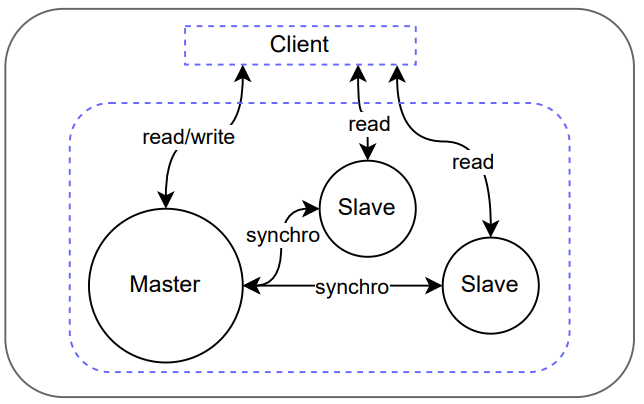
\includegraphics[width=0.5\textwidth]{diagramas/maestro-esclavo.png}
    \end{center}
    
\end{frame}

\begin{frame}
    \frametitle{Sistemas Distribuidos - Modelo Maestro-Maestro}

    En este modelo todos los nodos en el sistema son tanto \textbf{Maestros} como \textbf{Esclavos}.

     

    La replicación de datos es bidireccional.

     

    Cada nodo es responsable de mantener una copia exacta de los datos y asegurar la sincronización.

     

    \begin{center}
        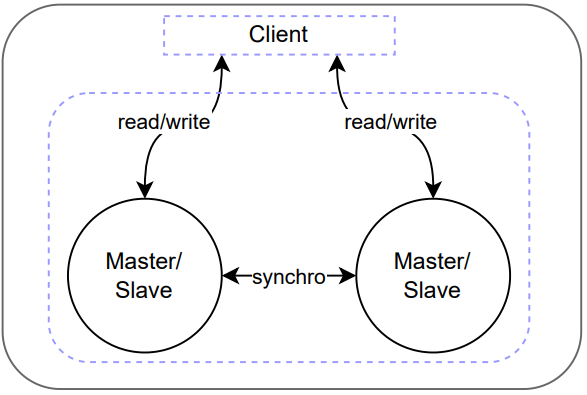
\includegraphics[width=0.5\textwidth]{diagramas/maestro-maestro.png}
    \end{center}
    
\end{frame}

\begin{frame}
    \frametitle{Sistemas Distribuidos - Modelos de Replicación}

    La principal diferencia entre los modelos, es que el modelo \textbf{Maestro-Esclavo} cuenta con un único nodo \textbf{Maestro}.

     

    Por lo que podemos decir que dicho modelo cuenta con un control \textit{Centralizado}.

     

    Este nodo se puede convertir en un cuello de botella.   Y además, si falla el nodo Maestro...   estamos en problemas.

     

    Igualmente, existen soluciones para este problema 
    
    \begin{enumerate}
        \item Tener uno o más nodos Maestros de backup.  
        \item Asignar hardware potente al nodo Maestro.  
        \item etc.
    \end{enumerate}

     

    Estas soluciones pueden combinarse.
    
\end{frame}

\begin{frame}
    \frametitle{Sistemas Distribuidos - Partición de Archivos}

    La Partición de Archivos es otra característica a tener en cuenta en los sistemas distribuidos.

     

    Se refiere a la división de la información en fragmentos que se distribuyen entre los nodos.

     

    Esta distribución mejora el rendimiento al permitir a su vez distribuir las consultas y hacer paralelismo. 

     

    Aumenta la resilencia del sistema debido a la redundancia de la información, si falla algún nodo, la información sigue disponible.
    
\end{frame}

\begin{frame}
    \frametitle{Sistemas Distribuidos - Acceso de Datos de Alto Desempeño}

    Generalmente se necesita encontrar un registro particular entre millones.

     

    El crecimiento de la información hace que esta búsqueda se ralentice.

     

    Aquí entra en juego el \textit{High Performance Data Access} (HPDA).

     

    Se refiere a la capacidad de un sistema para acceder y manipular grandes volúmenes de datos de manera rápida y eficiente.

     

    Se suelen utilizar técnicas de \textit{hashing} y/o particionado de rango sobre claves de valores.
    
\end{frame}

\begin{frame}
    \frametitle{Sistemas Distribuidos - Acceso de Datos de Alto Desempeño}

    \begin{itemize}
        \item \textbf{Hashing.}

        Esta técnica aplica una función de hash $h$ a una clave $K$.

         
    
        La aplicación $h(K)$ devuelve la ubicación del objeto en el sistema distribuido.

         
        
        \item \textbf{Particionado de rango sobre claves.} 

        Se asignan los valores a ubicaciones en función de un rango de valores de clave.

         

        Una ubicación $u$ podría tener los valores cuyas claves $K$ estén en el rango
        
        \begin{center}
            $Ku_{min} \leq K \leq Ku_{max}$
        \end{center}
        
    \end{itemize}
\end{frame}

\begin{frame}
    \frametitle{Sistemas Distribuidos - Conjetura de Brewer}

    También conocida como Teorema CAP.

     
    
    Las siglas \textbf{CAP} vienen de:

     

    \begin{itemize}
        \item \textit{\textbf{C}onsistency} (Consistencia)                        

        \item \textit{\textbf{A}vailability} (Disponibilidad)                     

        \item \textit{\textbf{P}artition Tolerance} (Tolerancia a Particiones)
        
    \end{itemize}

      
    
    Dicho Teorema enuncia lo siguiente

     
    
    \begin{Teorema}
    Dadas las propiedades \textbf{Consistencia}, \textbf{Disponibilidad} y \textbf{Tolerancia a Particiones}, solo se pueden cumplir dos de estas tres simultáneamente en un sistema distribuido.
    \end{Teorema}

     

    Los sistemas NoSQL, sacrifican la consistencia por \textit{consistencia eventual}, para garantizar en mayor medida disponibilidad y tolerancia a particiones.
    
\end{frame}

\section{Modelos de datos NoSQL}

\begin{frame}
    \frametitle{Clasificación}

    Existe una amplia variedad de modelos de datos \textit{NoSQL}. Entre los más conocidos encontramos:

     

    \begin{enumerate}
        \item Clave-Valor    
        \item Columnar        
        \item Documental     
        \item Grafo
    \end{enumerate}
\end{frame}

\subsection{Clave-Valor}

\indc{1}{0}{0}{0}

\subsection{Clave-Valor}

\begin{frame}
    \frametitle{Clave-Valor - Repaso}

    Este modelo almacena pares del tipo (\textit{Key}, \textit{Value}).
    
    \begin{center}
    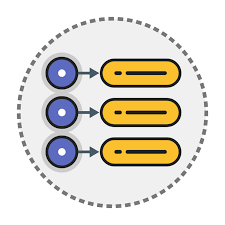
\includegraphics[width=0.2\textwidth]{images/KeyValue.png}
    \end{center}

     
    
     \begin{itemize}
        \item \textbf{Key}: Un identificador único para acceder al valor asociado.

         
        
         \item \textbf{Value}: Puede ser cualquier tipo de dato, desde texto, números y documentos, hasta listas o incluso otros pares clave-valor.
     \end{itemize}

\end{frame}

\begin{frame}
    \frametitle{Clave-Valor - Ejemplos}
    
    Algunas de las implementaciones más conocidas son:

     
    
     \begin{itemize}
        \item \textbf{Amazon DynamoDB}
                        
        \item \textbf{Voldemort}

        \item \textbf{Riak}
        
        \item \textbf{Redis}
     
     \end{itemize}

     

     Nos vamos a centrar en esta última.
\end{frame}

\subsubsection{Redis}

\begin{frame}   
    \frametitle{Clave-Valor - Redis}

    \textbf{Redis} significa ``\textbf{RE}mote \textbf{DI}ctionary \textbf{S}erver''

    \begin{center}
        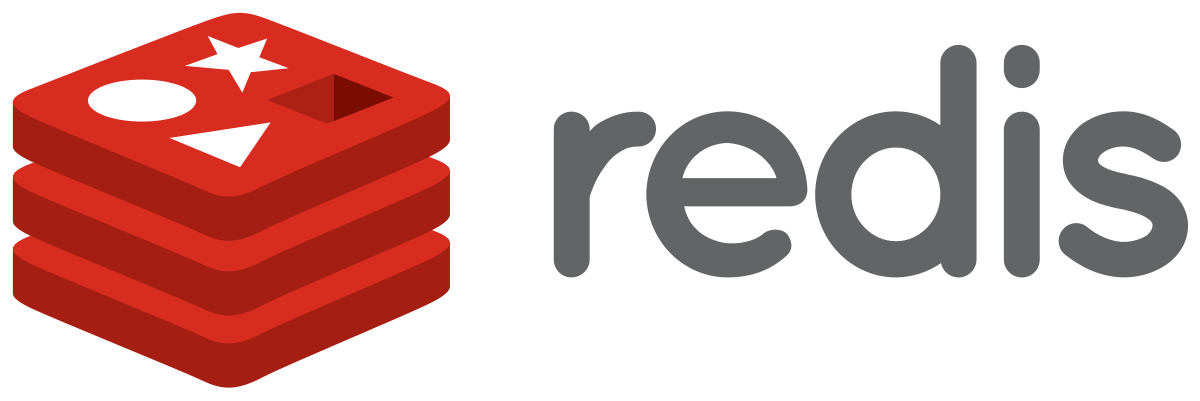
\includegraphics[width=0.3\textwidth]{images/redis_logo.png}
    \end{center}
    
     

    \begin{itemize}
        \item Base de datos de código abierto.  
        \item Rápida y versátil.  
        \item Diseñada como un almacén de estructuras de datos en memoria.
    \end{itemize}

\end{frame}

\begin{frame}
    \frametitle{Características de Redis}

    \begin{itemize}
        \item Estructuras de datos: strings, hashes, listas, conjuntos, etc.  
        \item Operaciones atómicas: Agregar, incrementar, intersección, unión, etc.  
        \item Replicación de datos incorporada.  
        \item Trabaja con un conjunto de datos en memoria.
    \end{itemize}
\end{frame}

\begin{frame}{Operaciones de Redis}
    
    Redis ofrece más de \textbf{400} operaciones e implementa la interfaz teórica para cada uno de los tipos de datos mencionados.
    
      

    Algunos ejemplos son:

      

    \begin{itemize}
        \item \textit{Strings:} $SET$, $GET$ y $DEL$
        
        \item \textit{Hashes:} $HSET$, $HGET$ y $HDEL$

        \item \textit{Listas:} $LPUSH$, $LPOP$, $RPUSH$, $RPOP$, $LRANGE$

        \item etc.
    \end{itemize}

\end{frame}

\begin{frame}{Ejemplo de Uso}
    \textbf{SET}: Agrega un par $(key, value)$.
    \begin{itemize}
        \item Complejidad temporal: $\mathcal{O}(1)$.
    \end{itemize}
    \vspace{0.6}
    \texttt{redis> SET subject1 "Base de Datos Avanzadas"} \newline
    \texttt{OK}   

\end{frame}
\begin{frame}{Ejemplo de Uso}
    \textbf{GET}: Obtiene el valor de una $key$.
    \begin{itemize}
        \item Complejidad temporal: $\mathcal{O}(1)$.
    \end{itemize}

    \texttt{redis> GET subject1}\newline
    \texttt{"Base de Datos Avanzadas"}

\end{frame}


\begin{frame}{Ejemplo de Uso}
    \textbf{LPUSH}: Inserta valores en la cabeza de una lista.
    \begin{itemize}
        \item Complejidad temporal: $\mathcal{O}(N)$.
    \end{itemize}
    
    \texttt{redis> LPUSH mylist "NoSQL"} \newline
    \texttt{redis> LPUSH mylist "Datos"} \texttt{"De"} \texttt{"Bases"}

\end{frame}
\begin{frame}{Ejemplo de Uso}
    \textbf{LRANGE}: Retorna los elementos en un rango especificado de una lista.
    \begin{itemize}
        \item Complejidad temporal: $\mathcal{O}(S + N)$.
    \end{itemize}
    \texttt{redis> LRANGE mylist 0 2} \newline
    \texttt{1) "Bases"} \newline
    \texttt{2) "De"} \newline
    \texttt{3) "Datos"} 
\end{frame}

\indc{0}{1}{0}{0}

\subsection{Columnar}

\begin{frame}
    \frametitle{Columnar}

    Las bases de datos orientadas a columnas almacenan datos verticalmente por columnas en lugar de horizontalmente por filas, permitiendo un acceso más eficiente a datos específicos.
    
    \begin{center}
        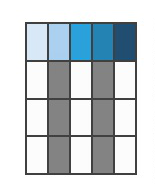
\includegraphics[width=0.3\textwidth]{diagramas/Columnar.png}
    \end{center}
\end{frame}


\begin{frame}
    \frametitle{Columnar - Ventajas}

    \begin{itemize}
        \item  Mayor eficiencia en consultas sobre columnas específicas.  
        \item  Convenientes para análisis de grandes volúmenes de datos.  
        \item  Adecuadas para aplicaciones de business intelligence y análisis predictivo.
    \end{itemize}
\end{frame}

\begin{frame}
    \frametitle{Columnar - Desventajas}
    \begin{itemize}
        \item  Operaciones de escritura más lentas debido a la reorganización de datos en columnas específicas.  
        \item  Posibles desafíos en entornos con datos altamente transaccionales.
    \end{itemize}
\end{frame}

\begin{frame}
    \frametitle{Columnar - Ejemplos}

    Algunos ejemplos de bases de datos columnares son: 
    
    \begin{itemize}
        \item \textbf{Apache Cassandra}\\
        Aunque es principalmente una base de datos de clave-valor, Cassandra utiliza un modelo de almacenamiento columnar para mejorar el rendimiento de ciertas consultas.  
        \item \textbf{Apache HBase}\\
        HBase es una base de datos de columnas distribuida, que almacena datos de forma columnar y permite un acceso eficiente a través de claves de fila.   
        \item \textbf{ClickHouse}\\
        ClickHouse es una base de datos de análisis columnar de código abierto diseñada para consultas analíticas de alto rendimiento en grandes conjuntos de datos.
    \end{itemize}
\end{frame}

\indc{0}{0}{1}{0}

\subsection{Documental}

\subsection{Documental}

\begin{frame}
    \frametitle{Documental}

    \begin{columns}
        \begin{column}{0.48\textwidth}
            Las bases de datos documentales almacenan datos en documentos individuales, que pueden ser estructurados o semi-estructurados como archivos JSON o XML.
        \end{column}
        \begin{column}{0.48\textwidth}
            \centering
            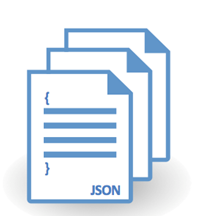
\includegraphics[width=0.5\textwidth]{images/Documental.png}
        \end{column}
    \end{columns}
    
     

    \vspace{0.3cm}
    
    Son especialmente adecuadas para aplicaciones donde los datos tienen una estructura flexible y variable como por ejemplo:

     
    
    \begin{itemize}
        \item \textbf{Contenido web}  
        \item \textbf{Análisis de registros}  
        \item \textbf{Gestión de datos de productos}
        \item etc.
    \end{itemize}
\end{frame}

\begin{frame}
    \frametitle{Documental - Ejemplos}

    Algunos ejemplos de bases de datos documentales son:
    
    \begin{itemize}
        \item \textbf{MongoDB}

        \item \textbf{CouchDB}
    \end{itemize}

     
    
    Nos vamos a centrar en MongoDB.
\end{frame}

\subsubsection{MongoDB}

\begin{frame}
    \frametitle{Documental - MongoDB}

        \centering
    
\includegraphics[width=0.4\textwidth]{images/mongodb-logo.png}
    \begin{itemize}
        \item Base de datos de código abierto, orientada a documentos y altamente escalable.  
        \item Desarrollada por MongoDB Inc.  
        \item Modelo de datos flexible basado en documentos BSON.  
        \item Utiliza almacenamiento basado en archivos de mapeo directo o motor WiredTiger.  
        \item Maneja replicación a través de conjuntos de réplicas para alta disponibilidad.  
        \item Distribuye datos en clústeres de servidores llamados fragmentos.  
        \item Lenguaje de consulta poderoso y flexible.
    \end{itemize}

\end{frame}

\begin{frame}[fragile]
\frametitle{Operaciones comunes en MongoDB}
\begin{itemize}
    \item \textbf{Insertar un documento}
    \begin{verbatim}
db.users.insertOne({
    name: "John Doe",
    age: 30,
    email: "john@example.com"
})

db.users.insertMany([
  { name: "Alice", age: 25 },
  { name: "Bob", age: 30 },
  { name: "Charlie", age: 50 }
])
    \end{verbatim}

\end{itemize}
\end{frame}

\begin{frame}[fragile]
\frametitle{Operaciones comunes en MongoDB}
\begin{itemize}
    \item \textbf{Consultar documentos}
    \begin{verbatim}
db.users.find({ age: { $gt: 25 } })
    \end{verbatim}

     
    \item \textbf{Actualizar documentos}
    \begin{verbatim}
db.users.updateOne(
    { name: "John Doe" },
    { $set: { age: 35 } }
)

db.users.updateMany(
    { status: "active" }, 
    { $set: { status: "inactive" } }
)

    \end{verbatim}
\end{itemize}
\end{frame}

\begin{frame}[fragile]
\frametitle{Operaciones comunes en MongoDB}
\begin{itemize} 
    \item \textbf{Eliminar documentos}
    \begin{verbatim}
db.users.deleteOne({ name: "John Doe" })
db.users.deleteMany({ age: { $gt: 40 } })
    \end{verbatim}
         
    \item \textbf{Contar documentos}
\begin{verbatim}
db.users.countDocuments({ age: { $lt: 30 } })
\end{verbatim}
         
    \item \textbf{Valores Distintos}
\begin{verbatim}
db.users.distinct("city", { country: "USA" })
\end{verbatim}
         
    \item \textbf{Agregar datos}
\begin{verbatim}
db.sales.aggregate([
  { $match: { status: "completed" } },
  { $group: { _id: "$product", 
            totalAmount: { $sum: "$amount" } } }
])
\end{verbatim}

\end{itemize}

\end{frame}

\indc{0}{0}{0}{1}

\subsection{Grafo}

\subsection{Grafo}

\begin{frame}
    \frametitle{Grafo - Repaso}

    Las bases de datos en grafo utilizan estructuras de grafo para almacenar, consultar y relacionar datos. 

     
    
    \begin{columns}
        \begin{column}{0.48\textwidth}
            Los datos se representan mediante nodos (entidades) y arcos (relaciones entre entidades).
        \end{column}
        \begin{column}{0.48\textwidth}
            \centering
            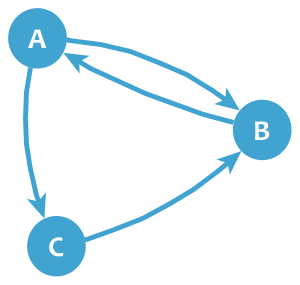
\includegraphics[width=0.4\textwidth]{images/Grafo.png}
        \end{column}
    \end{columns}

     

    \vspace{0.3cm}
    
    Pueden asignarse propiedades a nodos y arcos para capturar más detalles.

     
    
    Son ideales para almacenar datos interconectados.  

     
    
    Aplicaciones comunes incluyen: \textbf{Redes sociales}, \textbf{Sistemas de recomendación}, \textbf{Redes de trasportes}, etc.

    
\end{frame}

\begin{frame}
    \frametitle{Grafo - Ejemplos}

    Algunos ejemplos de bases de datos en grafos son:

    \begin{itemize}
        \item \textbf{Neo4j}\\
         
        \item \textbf{GraphBase}\\ 

        \item \textbf{Infinite Graph}\\
        
        \item \textbf{FlockDB}\\
    \end{itemize}
    
     

    Nos vamos a centrar en Neo4j.
    
\end{frame}

\subsubsection{Neo4j}

\begin{frame}
    \frametitle{Grafo - Neo4j}

    \centering
    
\includegraphics[width=0.5\textwidth]{images/neo4j-logo.png}

    \begin{itemize}
        \item Plataforma líder en bases de datos de grafos.  
        \item Diseño nativo de grafo para un rendimiento óptimo y escalabilidad excepcional.  
        \item Utiliza Cypher como su lenguaje de consulta principal.  
        \item Ofrece una interfaz integrada de visualización de grafos.  
        \item Altamente escalable y diseñado para manejar grandes volúmenes de datos.  
        \item Garantiza propiedades ACID.  
        \item Edición empresarial.
    \end{itemize}
    
\end{frame}

\begin{frame}{Cypher: Lenguaje de Consulta de Neo4j}
    \begin{itemize}
        \item Sintaxis intuitiva y expresiva.  
        \item Orientado a patrones.  
        \item Declarativo.  
        \item Soporte completo para operaciones CRUD.  
        \item Amplio soporte para funciones y operadores para operaciones avanzadas.
    \end{itemize}
\end{frame}

\begin{frame}
    \frametitle{Operaciones Básicas de Neo4j}

    Estas son algunas de las cláusulas básicas más comunes en Cypher y su sintaxis asociada:

     

    \begin{itemize}
        \item \textbf{Crear nodos y relaciones}

        \texttt{CREATE (a:Person \{name: 'John', age: 30\})} \newline
         
        \texttt{CREATE (b:Person:Employee 
                            \{name: 'Alice', role: 'Manager'\})}\newline
         
        \texttt{CREATE (a)-[:FRIENDS\_WITH]->(b)}

         
            
        \item \textbf{Especificar patrones}
        
        \texttt{MATCH (p:Person \{name: 'John'\}) RETURN p}\newline
         
        \texttt{MATCH (p:Person \{name: 'John'\})-[r]->() RETURN p, r}

         
    
    
        \item \textbf{Filtrar resultados}

        \texttt{WHERE n.name = 'John' AND friend.age > 25}

 
    \end{itemize}
    
\end{frame}

\begin{frame}
    \frametitle{Operaciones Básicas de Neo4j}


    \begin{itemize}

     
        \item \textbf{Devolver datos}

        \texttt{RETURN n, friend}

         
         
        \item \textbf{Actualizar propiedades}

        \texttt{SET n.age = 30}

         
        
        \item \textbf{Eliminar nodos y relaciones.}

        \texttt{DELETE n, friend}

         
            
        \item \textbf{Ordenar resultados}

        \texttt{ORDER BY n.name DESC}

         
        
        \item \textbf{Limitar número de resultados}

        \texttt{LIMIT 10}

         

        \item \textbf{Crear índices}

        \texttt{CREATE INDEX ON :Person(name)}
    
        
    \end{itemize}
    
\end{frame}

\begin{frame}[fragile]
  \frametitle{Ejemplo de Consulta en Neo4j}
      Para una demostración de como estas operaciones podrían ser utilizadas, supongamos que queremos encontrar los amigos en común entre dos usuarios en una red social y alguna información adicional sobre esos amigos en común:  
    \begin{verbatim}
MATCH (userA:User {username: 'UsuarioA'})
    -[:FRIENDS_WITH]-(commonFriend)-[:FRIENDS_WITH]-
    (userB:User {username: 'UsuarioB'})
RETURN commonFriend.username AS commonFriendUsername,
       commonFriend.age AS commonFriendAge
    \end{verbatim}

        
\end{frame}

\begin{frame}{Empresas que Utilizan Neo4j}
    \begin{itemize}
        \item Walmart
        \item Volvo
        \item eBay
        \item Cisco
    \end{itemize}
\end{frame}

\begin{frame}
    \frametitle{}
    \begin{center}
    	¿Dudas?
    \end{center}
\end{frame}

\begin{frame}
\frametitle{Referencias}
    \begin{itemize}
    	\item N. Reyes, O. E. Gagliardi, C. Deco, and M. T. Taranilla. \textit{Bases de Datos, Maestría en Tecnología de la Información}. 2018.
    
        \item C. M. Bender, C. Deco, J. S. González, M. Hallo, and J. C. Ponce Gallegos. \textit{Tópicos Avanzados de Bases de Datos}. 2014.

        \item E. Gómez and L. Mota. \textit{Introducción a las bases de datos NoSQL. Sistemas de bases de datos orientados a grafos}. 2021.
    \end{itemize}
\end{frame}

\end{document}